\documentclass[noinstructornotes]{ximera}
%handout:  for handout version with no solutions or instructor notes
%handout,instructornotes:  for instructor version with just problems and notes, no solutions
%noinstructornotes:  shows only problem and solutions

%% handout
%% space
%% newpage
%% numbers
%% nooutcomes

%I added the commands here so that I would't have to keep looking them up
%\newcommand{\RR}{\mathbb R}
%\renewcommand{\d}{\,d}
%\newcommand{\dd}[2][]{\frac{d #1}{d #2}}
%\renewcommand{\l}{\ell}
%\newcommand{\ddx}{\frac{d}{dx}}
%\everymath{\displaystyle}
%\newcommand{\dfn}{\textbf}
%\newcommand{\eval}[1]{\bigg[ #1 \bigg]}

%\begin{image}
%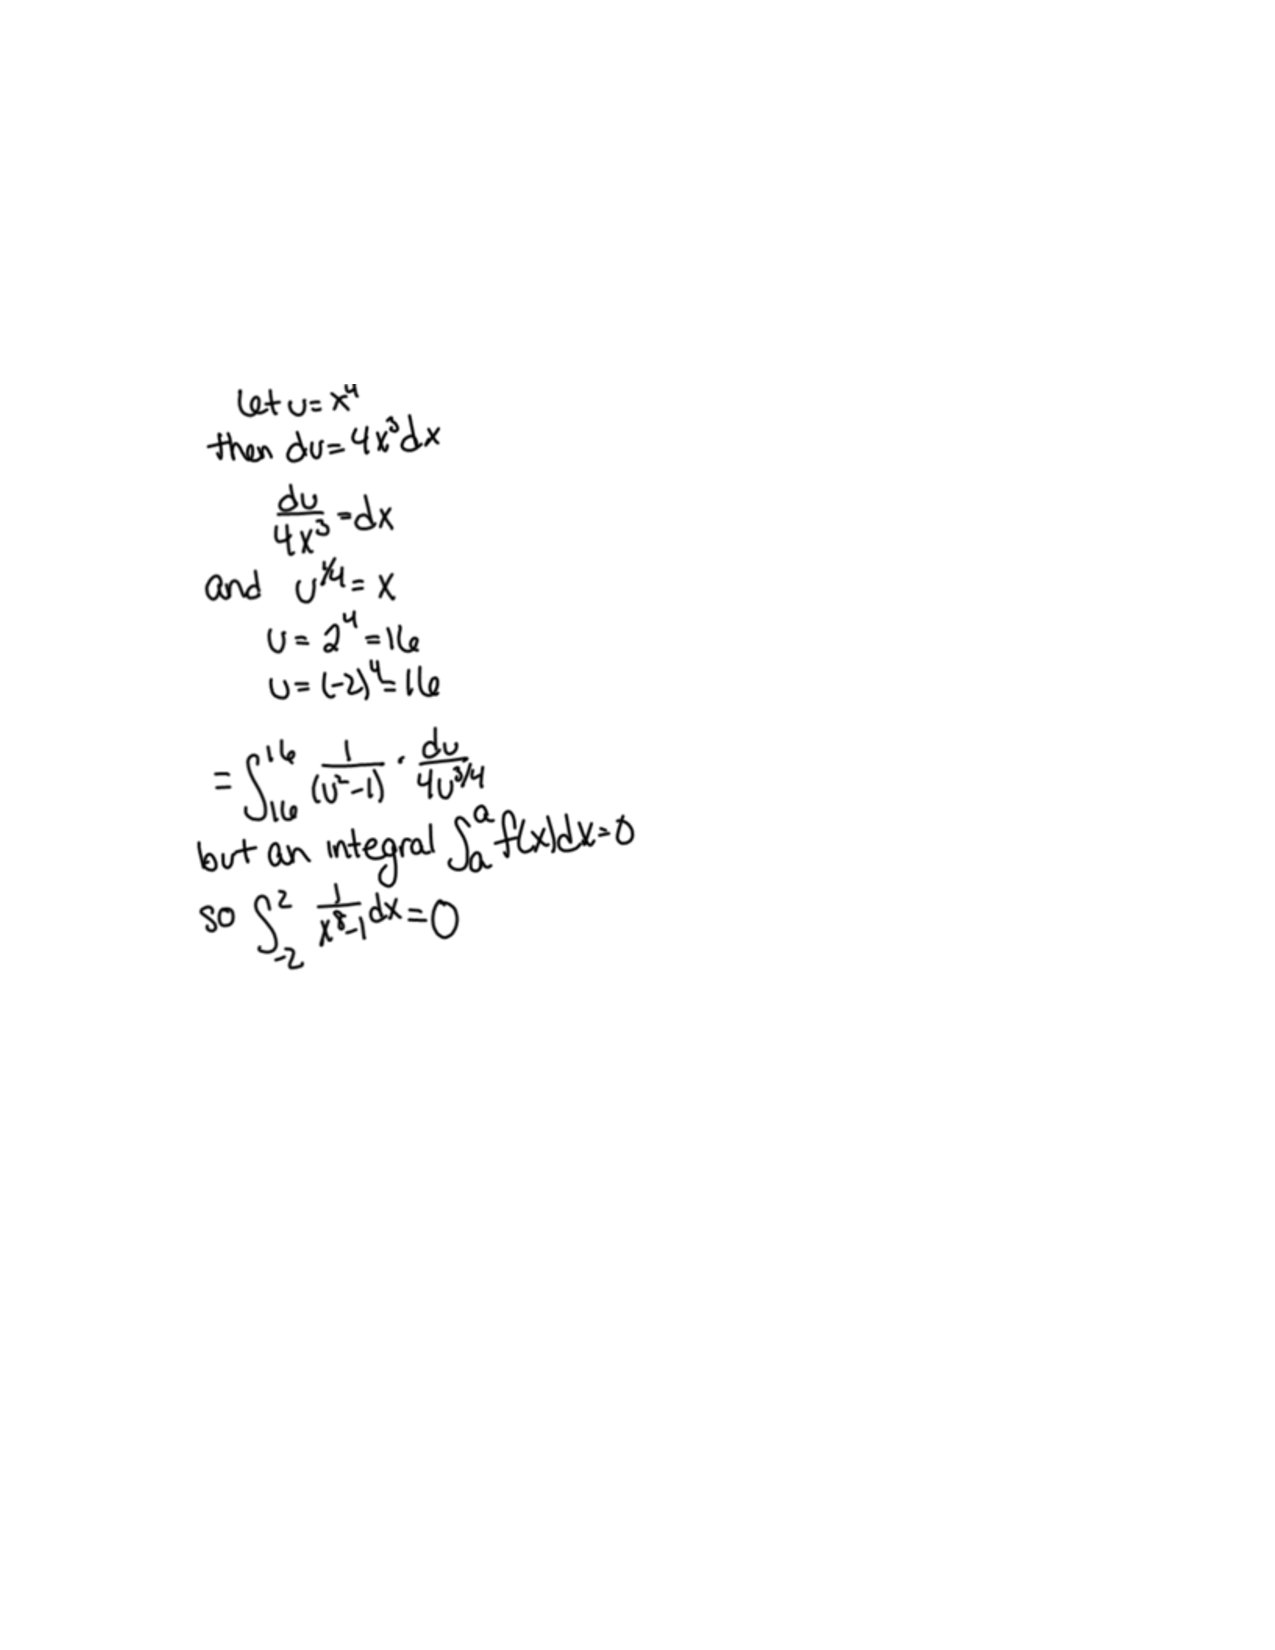
\includegraphics[trim= 170 420 250 180]{Figure1.pdf}
%\end{image}

%add a ``.'' below when used in a specific directory.
\newcommand{\RR}{\mathbb R}
\renewcommand{\d}{\,d}
\newcommand{\dd}[2][]{\frac{d #1}{d #2}}
\renewcommand{\l}{\ell}
\newcommand{\ddx}{\frac{d}{dx}}
\newcommand{\dfn}{\textbf}
\newcommand{\eval}[1]{\bigg[ #1 \bigg]}

\usepackage{multicol}

\renewenvironment{freeResponse}{
\ifhandout\setbox0\vbox\bgroup\else
\begin{trivlist}\item[\hskip \labelsep\bfseries Solution:\hspace{2ex}]
\fi}
{\ifhandout\egroup\else
\end{trivlist}
\fi} %% we can turn off input when making a master document

\title{Recitation \# 5:  Length of Curves \& Surface Area - Solutions}  

\begin{document}
\begin{abstract}		\end{abstract}
\maketitle



\begin{comment}
\section{Warm up:}

	\begin{freeResponse}
	
	\end{freeResponse}
	
\begin{instructorNotes}

\end{instructorNotes}
\end{comment}







\section{Group work:}



%problem 1





%problem 1
\begin{problem}
Find the length of the following curves (length is in feet):
	\begin{enumerate}
		\item  $y = \frac{1}{6} x^3 + \frac{1}{2x}$ from $\left( 2, \frac{19}{12} \right)$ to $\left( 3, \frac{14}{3} \right)$.  
		\begin{freeResponse}
			\begin{align*}
			\text{{\color{red} Arc Length}} &= \int_2^3 \sqrt{1+y'(x)^2} \d x  \\
			&= \int_2^3 \sqrt{1+ \left( \frac{1}{2}x^2 - \frac{1}{2}x^{-2} \right)^2} \d x  \\
			&= \int_2^3 \sqrt{1+ \left( \frac{1}{4}x^4 - \frac{1}{2} + \frac{1}{4}x^{-4} \right)} \d x  \\
			&= \int_2^3 \sqrt{\frac{1}{4}x^4 + \frac{1}{2} + \frac{1}{4}x^{-4}} \d x  \\
			&= \int_2^3 \sqrt{\left( \frac{1}{2}x^2 + \frac{1}{2}x^{-2} \right)^2} \d x  \\
			&= \int_2^3 \left( \frac{1}{2}x^2 + \frac{1}{2}x^{-2} \right) \d x  \\
			&= \eval{\frac{1}{6}x^3 - \frac{1}{2x}}_2^3  \\
			&= \left( \frac{27}{6} - \frac{1}{6} \right) - \left( \frac{8}{6} - \frac{1}{4} \right)  \\
			&= 3 + \frac{1}{4} = \frac{13}{4}.
			\end{align*}
		\end{freeResponse}
		
		
		
		\item  $x = \frac{1}{9} e^{3y} + \frac{1}{4} e^{-3y}$ from $\left( \frac{13}{36}, 0 \right)$ to $\left( \frac{265}{288}, \ln 2 \right)$.  
		\begin{freeResponse}
			\begin{align*}
			\text{{\color{red} Arc Length}} &= \int_0^{\ln 2} \sqrt{1+x'(y)^2} \d y  \\
			&=\int_0^{\ln 2} \sqrt{1+ \left( \frac{1}{3}e^{3y} - \frac{3}{4}e^{-3y} \right)^2} \d y  \\
			&=  \int_0^{\ln 2} \sqrt{1+ \left( \frac{1}{9}e^{6y} - \frac{1}{2} + \frac{9}{16}e^{-6y} \right)} \d y  \\
			&= \int_0^{\ln 2} \sqrt{ \frac{1}{9}e^{6y} + \frac{1}{2} + \frac{9}{16}e^{-6y} } \d y  \\
			&= \int_0^{\ln 2} \sqrt{ \left( \frac{1}{3}e^{3y} + \frac{3}{4}e^{-3y} \right)^2} \d y  \\
			&= \int_0^{\ln 2} \left( \frac{1}{3}e^{3y} + \frac{3}{4}e^{-3y} \right) \d y  \\
			&= \eval{ \frac{1}{9}e^{3y} - \frac{1}{4}e^{-3y}}_0^{\ln 2}  \\
			&\overset{*}{=} \left( \frac{8}{9} - \frac{1}{32} \right) - \left( \frac{1}{9} - \frac{1}{4} \right)  \\
			&= \frac{7}{9} + \frac{7}{32} = \frac{224 + 63}{288} = \frac{287}{288}.
			\end{align*}
		* Note that
			\[
			e^{3 \ln 2} = e^{\ln 2^3} = e^{\ln 8} = 8
			\]
	and
			\[
			e^{-3 \ln 2} = e^{\ln 2^{-3}} = 2^{-3} = \frac{1}{8}.
			\]
		\end{freeResponse}
		
	\end{enumerate}

\end{problem}

\begin{instructorNotes}
Split (a) and (b) amont the groups.  
Note that the focus here is on both the set-up \dfn{and} in solving the resulting integral (which boild down to writing the expression under the radical as a perfect square).
\end{instructorNotes}



%problem 2
\begin{problem}
Find the surface area of the surface generated by revolving the curve given by
	\begin{enumerate}
		\item  $y = \frac{1}{6} x^3 + \frac{1}{2x}$ from $\left( 2, \frac{19}{12} \right)$ to $\left( 3, \frac{14}{3} \right)$ about the $x$-axis.
		\begin{freeResponse}
		The formula for the surface area is
			\[
			\text{{\color{red} Surface Area}} = \int_2^3 2 \pi f(x) \sqrt{1+f'(x)^2} \d x.
			\]
		Since $y = f(x) = \frac{1}{6} x^3 + \frac{1}{2x}$, we know that $f'(x) = \frac{1}{2} x^2 - \frac{1}{2} x^{-2}$.  
		Note that
			\begin{align*}
			\sqrt{1+f'(x)^2} &= \sqrt{1+ \left( \frac{1}{2}x^2 - \frac{1}{2}x^{-2} \right)^2}  \\
			&= \sqrt{1+ \left( \frac{1}{4}x^4 - \frac{1}{2} + \frac{1}{4}x^{-4} \right)}  \\
			&= \sqrt{\frac{1}{4}x^4 + \frac{1}{2} + \frac{1}{4}x^{-4}}  \\
			&= \sqrt{\left( \frac{1}{2}x^2 + \frac{1}{2}x^{-2} \right)^2}  \\
			&= \left( \frac{1}{2}x^2 + \frac{1}{2}x^{-2} \right)
			\end{align*}
		and so
			\begin{align*}
			\text{{\color{red} Surface Area}} &= \int_2^3 2 \pi \left( \frac{1}{6} x^3 + \frac{1}{2} x^{-1} \right) \left( \frac{1}{2} x^2 + \frac{1}{2} x^{-2} \right) \d x  \\
			&= 2 \pi \int_2^3 \left( \frac{1}{12} x^5 + \frac{1}{12} x + \frac{1}{4} x + \frac{1}{4} x^{-3} \right) \d x  \\
			&= 2 \pi \int_2^3 \left( \frac{1}{12} x^5 + \frac{1}{3} x + \frac{1}{4} x^{-3} \right) \d x  \\
			&= 2 \pi \eval{\frac{1}{72}x^6 + \frac{1}{6}x^2 - \frac{1}{8}x^{-2}}_2^3  \\
			&= 2\pi \left[ \left( \frac{81}{8} + \frac{3}{2} - \frac{1}{72} \right) - \left( \frac{8}{9} + \frac{2}{3} - \frac{1}{32} \right) \right]  \\
			&= 2\pi \left( \frac{2916 + 432 - 4 - 256 - 192 + 9}{288} \right)  \\
			&= \frac{2905 \pi}{144}.
			\end{align*}
		\end{freeResponse}
		
		
		
		\item  $x = \frac{1}{9} e^{3y} + \frac{1}{4} e^{-3y}$ from $\left( \frac{13}{36}, 0 \right)$ to $\left( \frac{265}{288}, \ln 2 \right)$ about the $y$-axis.
		\begin{freeResponse}
		The formula for the surface area is
			\[
			\text{{\color{red} Surface Area}} = \int_0^{\ln 2} 2 \pi f(y) \sqrt{1+f'(y)^2} \d y.
			\]
		Since $x = f(y) = \frac{1}{9} e^{3y} + \frac{1}{4} e^{-3y}$, 
		we know that $f'(y) = \frac{1}{3} e^{3y} - \frac{3}{4} e^{-3y}$.  
		Note that
			\begin{align*}
			\sqrt{1+f'(y)^2} \d y  &= \sqrt{1+ \left( \frac{1}{3}e^{3y} - \frac{3}{4}e^{-3y} \right)^2}  \\
			&=  \sqrt{1+ \left( \frac{1}{9}e^{6y} - \frac{1}{2} + \frac{9}{16}e^{-6y} \right)}  \\
			&= \sqrt{ \frac{1}{9}e^{6y} + \frac{1}{2} + \frac{9}{16}e^{-6y} }   \\
			&= \sqrt{ \left( \frac{1}{3}e^{3y} + \frac{3}{4}e^{-3y} \right)^2}  \\
			&= \frac{1}{3}e^{3y} + \frac{3}{4}e^{-3y}
			\end{align*}
		and so
			\begin{align*}
			\text{{\color{red} Surface Area}} &= \int_0^{\ln 2} 2 \pi \left( \frac{1}{9} e^{3y} + \frac{1}{4} e^{-3y} \right) \left( \frac{1}{3}e^{3y} + \frac{3}{4}e^{-3y} \right) \d y  \\
			&= 2 \pi \int_0^{\ln 2} \left( \frac{1}{27}e^{6y} + \frac{1}{6} + \frac{3}{16}e^{-6y} \right) \d y  \\
			&= 2 \pi \eval{\frac{1}{162}e^{6y} + \frac{1}{6}y - \frac{1}{32}e^{-6y}}_0^{\ln 2}  \\
			&= 2 \pi \left[ \left( \frac{32}{81} + \frac{\ln 2}{6} - \frac{1}{2048} \right) - \left( \frac{1}{162} + 0 - \frac{1}{32} \right) \right]  \\
			&= \frac{\pi}{3} \left( \frac{9655}{3072} + \ln 2 \right).
			\end{align*}
		\end{freeResponse}
		
	\end{enumerate}
	
\end{problem}

\begin{instructorNotes}
Split (a) and (b) among the same groups as before.  
Make sure that the students are using the surface area formula and not the arc length formula.
\end{instructorNotes}
















	
	
	
	
	
	
	
	
	

	










								
				
				
	














\end{document} 


















